%% line1.tex
\documentclass{standalone}
\usepackage{tkz-euclide}
\usetkzobj{all}
%% ================== commands ==========================
\newcommand{\myShowPoints}[2]{
\tkzDrawPoints(#1) 
\tkzLabelPoints[#2](#1)
}		
\newcommand{\myGetMidPoint}[3]{
\tkzDefMidPoint(#1,#2)\tkzGetPoint{#3}
}		
\begin{document}
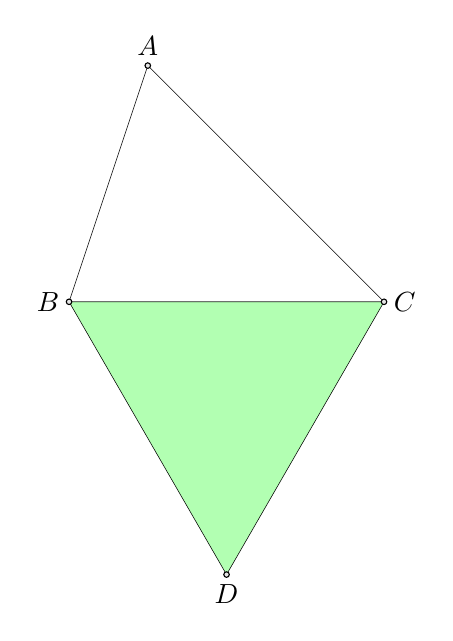
\begin{tikzpicture}
	\tkzDefPoints{0/0/B, 4/0/C, 1/3/A}
	% connecting 3 points
	\tkzDrawPolygon(A,B,C)
	% equilateral triangles
	\tkzDefTriangle[equilateral](C,B) \tkzGetPoint{D}
	\tkzDrawPolygon[fill=green!30](B,C,D)

	\tkzLabelPoints[below](D)
	\tkzLabelPoints[right](C)
	\tkzLabelPoints[above](A)
	\tkzLabelPoints[left](B)
	\tkzDrawPoints(A,B,C,D)
\end{tikzpicture}
\end{document}